\chapter{Fejlesztői dokumentáció}
\label{ch:impl}

A főprogram (betanított modell használata) alapvetően nézet-modell
architektúrát követ.

\section{Felhasználói felület}
A grafikus és a konzolos felhasználói felületek a \texttt{ui} könyvtárban
érhetőek el. A konzolos interfész egy nagyon egyszerű kommunikációt biztosít:
bekéri a felhasználótól a fájl nevét, majd az eredményt struktúrálva kiírja
a konzolra.

A grafikus felület ezzel szemben komplexebb. Az implementálás során
a \texttt{PySimpleGUI}\cite{??} könyvtárat használtam, melynek segítségével
könnyen lehet grafikus felületű alkalmazásokat készíteni Python nyelven.
A \texttt{GUI} osztály konstruktorában történik meg a felhasználói felület
elemeinek létrehozása, melyek a következők:
\begin{itemize}
    \item 2 Szövegdoboz (\texttt{Multiline}): a baloldali jeleníti meg az
    eredeti Assembly kódot, a jobboldali a visszafejtés 3 lépését:
    a szegmentált Assembly-t, a maszkolt C és a rekonstruált C-t.
    \item Szövegbeviteli mező (\texttt{TextInput}): Itt lehet megadni
    a betölteni kívánt fájl nevét. Ez alapvetően inaktív, a szövegbevitelt egy
    fájlkereső biztosítja.
    \item Fájlkereső (\texttt{FileBrowswer}):
    \item Gomb (\texttt{Button}): 
\end{itemize}

\begin{figure}[H]
	\centering
	\usetikzlibrary{trees}
\tikzstyle{every node}=[draw=black,thick,anchor=west]
\tikzstyle{file}=[draw=red]
\tikzstyle{optional}=[dashed,fill=gray!20]
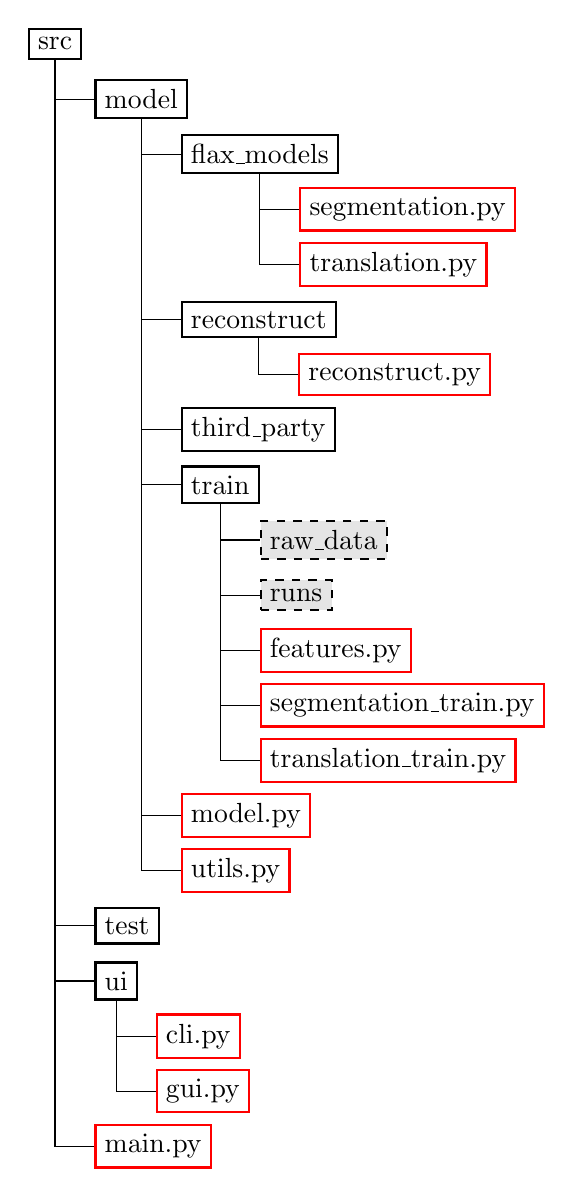
\begin{tikzpicture}[%
  grow via three points={one child at (0.5,-0.7) and
  two children at (0.5,-0.7) and (0.5,-1.4)},
  edge from parent path={(\tikzparentnode.south) |- (\tikzchildnode.west)}]
  \node {src}
    child { node {model}
      child { node {flax\_models}
        child { node [file] {segmentation.py}}
        child { node [file] {translation.py}}
      }
      child [missing] {}
      child [missing] {}
      child { node {reconstruct}
        child {node [file] {reconstruct.py}}
      }
      child [missing] {}
      child { node {third\_party}}
      child { node {train}
        child { node [optional] {raw\_data}}
        child { node [optional] {runs}}
        child { node [file] {features.py}}
        child { node [file] {segmentation\_train.py}}
        child { node [file] {translation\_train.py}}
      }
      child [missing] {}
      child [missing] {}
      child [missing] {}
      child [missing] {}
      child [missing] {}
      child { node [file] {model.py}}
      child { node [file] {utils.py}}
    }
    child [missing] {}				
    child [missing] {}				
    child [missing] {}
    child [missing] {}
    child [missing] {}
    child [missing] {}
    child [missing] {}
    child [missing] {}
    child [missing] {}
    child [missing] {}
    child [missing] {}
    child [missing] {}
    child [missing] {}
    child [missing] {}
    child { node {test}}
    child { node {ui}
      child {node [file] {cli.py}}
      child {node [file] {gui.py}}
    }
    child [missing] {}
    child [missing] {}
    child { node [file] {main.py}};
\end{tikzpicture}
	\caption{A kódbázis felépítése}
	\label{fig:file-system}
\end{figure}

\section{Gépi tanulási modellek}

\subsection{Jax \& Flax}
Ma már rengeteg különböző magas szintű könyvtár érhető el a \texttt{Python} nyelvhez, melyek 
megkönnyítik a mélytanulási algoritmusok implementálást. Én ezek közül a Google által fejlesztett \texttt
{Jax}-et\cite{jax2018github} és az arra épülő \texttt{Flax}-et\cite{flax2020github} használtam.

A Jax könyvtár két legfőbb komponense a gyorsított lineáris algebra (\texttt{XLA}) és az automatikus 
differenciálás. Mindkettő nagyban hozzájárul ahhoz, hogy könnyebben és gyorsabban lehessen különböző 
gépi tanulási algoritmusokat és modelleket implementálni, ezzel gyorsítva az ezirányú kutatásokat.

A gépi tanulási algoritmusok során nagyon sok lineáris algebrai műveletet (pl. mátrixszorzás) kell 
végezni, így elenghetetlen, hogy ezeket minél gyorsabban elvégezzük. Ebben segít az \texttt{XLA}, ami 
egy doménspecifikus fordító, célja, segítségével a lineáris algebrai műveletek elvé 

\subsection{tanítási folyamat}
A tanítási folyamat leírását a \texttt{model/train/training.py} fájl
taralmazza. A szegmentálás és a fordítás tanítása során is ezen modul
metódusait hívja a program.

A \texttt{train\_step} metódus egy tanítási lépés folyamatát írja le.
